\documentclass[12pt]{article}
\usepackage[top=1in, bottom=1in, left=.75in, right=.75in]{geometry}
\usepackage{amsmath, enumerate}
\usepackage{fancyhdr}
\usepackage{graphicx, xcolor, setspace}
\usepackage{txfonts}
\usepackage{multicol,coordsys,pgfplots}
\usepackage[scaled=0.86]{helvet}
\renewcommand{\emph}[1]{\textsf{\textbf{#1}}}
\usepackage{anyfontsize}
% \usepackage{times}
% \usepackage[lf]{MinionPro}
\usepackage{tikz,pgfplots}
%\def\degC{{}^\circ{\rm C}}
\def\ra{\rightarrow}
\usetikzlibrary{calc,arrows.meta}
\pgfplotsset{compat = newest}
\newcommand{\blank}[1]{\rule{#1}{0.75pt}}

\pgfplotsset{my style/.append style={axis x line=middle, axis y line=
middle, xlabel={$x$}, ylabel={$y$}}}

%axis equal

%yticklabels={,,} , xticklabels={,,}

% \setmainfont{Times}
% \def\sansfont{Lucida Grande Bold}
\parindent 0pt
\parskip 4pt
\pagestyle{fancy}
\fancyfoot[C]{\emph{\thepage}}
\fancyfoot[R]{v1}
\fancyhead[L]{\ifnum \value{page} > 1\relax\emph{Math F251X: Midterm 1}\fi}
\fancyhead[R]{\ifnum \value{page} > 1\relax\emph{Spring 2024}\fi}
\headheight 15pt
\renewcommand{\headrulewidth}{0pt}
\renewcommand{\footrulewidth}{0pt}
\let\ds\displaystyle
\def\continued{{\emph {Continued....}}}
\def\continuing{{\emph {Problem \arabic{probcount} continued....}}\par\vskip 4pt}


\newcounter{probcount}
\newcounter{subprobcount}
\newcommand{\thesubproblem}{\emph{\alph{subprobcount}.}}
\def\problem#1{\setcounter{subprobcount}{0}%
\addtocounter{probcount}{1}{\emph{\arabic{probcount}.\hskip 1em(#1)}}\par}
\def\subproblem#1{\par\hangindent=1em\hangafter=0{%
\addtocounter{subprobcount}{1}\thesubproblem\emph{#1}\hskip 1em}}
\def\probskip{\vskip 10pt}
\def\medprobskip{\vskip 2in}
\def\subprobskip{\vskip 45pt}
\def\bigprobskip{\vskip 4in}


\newenvironment{subproblems}{%
\begin{enumerate}%
\setcounter{enumi}{\value{subprobcount}}%
\renewcommand{\theenumi}{\emph{\alph{enumi}}}}%
{\setcounter{subprobcount}{\value{enumi}}\end{enumerate}}


\newcommand{\be}{\begin{enumerate}}
\newcommand{\ee}{\end{enumerate}}


\begin{document}
{\emph{\fontsize{26}{28}\selectfont Spring 2024 \hfill
%{\fontsize{32}{36}\selectfont Calculus 1: Midterm 1}
\hfill Math F251X}}

\begin{center}
{\emph{%\fontsize{26}{28}\selectfont Spring 2024 
%%\hfill
{\fontsize{32}{36}\selectfont Calculus 1: Midterm 1}
%%\hfill Math F251X}
}}
\end{center}

%\vskip 2cm
\strut\vtop{\halign{\emph#\hskip 0.5em\hfil&#\hbox to 2in{\hrulefill}\cr
\emph{\fontsize{18}{22}\selectfont Name:}&\cr
%\noalign{\vskip 10pt}
%\emph{\fontsize{18}{22}\selectfont Student Id:}&\cr
%\noalign{\vskip 10pt}
%\emph{\fontsize{18}{22}\selectfont Calculator Model:}&\cr
}}
\hfill
\vtop{\halign{\emph{\fontsize{18}{22}\selectfont #}\hfil& \emph{\fontsize{18}{22}\selectfont\hskip 0.5ex $\square$ #}\hfil\cr
Section: & 9:15am (James Gossell)\cr
\noalign{\vskip 4pt}
         & 11:45am (Mohamed Nouh)\cr
\noalign{\vskip 4pt}
         & async (Leah Berman)\cr}}

\vfill
{\fontsize{18}{22}\selectfont\emph{Rules:}}

\begin{itemize}
\item Partial credit will be awarded, but you must show your work.

\item You may have a single handwritten $3'' \times 5''$ notecard, both sides.

\item Calculators are {\bf not} allowed. 

\item Place a box around your  \fbox{FINAL ANSWER} to each question where appropriate.

\item Turn off anything that might go beep during the exam.

\end{itemize}

%If you need extra space, you can use the back sides of the pages.
%Please make it obvious  when you have done so.



Good luck!
\vfill
\def\emptybox{\hbox to 2em{\vrule height 16pt depth 8pt width 0pt\hfil}}
\def\tline{\noalign{\hrule}}
\centerline{\vbox{\offinterlineskip
{
\bf\sf\fontsize{18pt}{22pt}\selectfont
\hrule
\halign{
\vrule#&\strut\quad\hfil#\hfil\quad&\vrule#&\quad\hfil#\hfil\quad
&\vrule#&\quad\hfil#\hfil\quad&\vrule#\cr
height 3pt&\omit&&\omit&&\omit&\cr
&Problem&&Possible&&Score&\cr\tline
height 3pt&\omit&&\omit&&\omit&\cr
&1&&16&&\emptybox&\cr\tline
&2&&12&&\emptybox&\cr\tline
&3&&10&&\emptybox&\cr\tline
&4&&12&&\emptybox&\cr\tline
&5&&12&&\emptybox&\cr\tline
&6&&8&&\emptybox&\cr\tline
&7&&10&&\emptybox&\cr\tline
&8&&12&&\emptybox&\cr\tline
&9&&8&&\emptybox&\cr\tline \tline
&Extra Credit&&5&&\emptybox&\cr\tline
&Total&&100&&\emptybox&\cr
}\hrule}}}

\newpage
%\begin{enumerate}
%%%%



%\item (11 points) \textcolor{red}{( or 20 points)} 
\problem{16 points} The entirety of a function $H(x)$ is shown below. Use the graph of $H(x)$ to answer each question below. If a limit is infinite, indicate that with $\infty$ or $-\infty.$ If a value does not exist or is undefined, write {\bf DNE}.\\

%% 2 pts for the limit questions, 1 pt else. Or something like that

\begin{center}
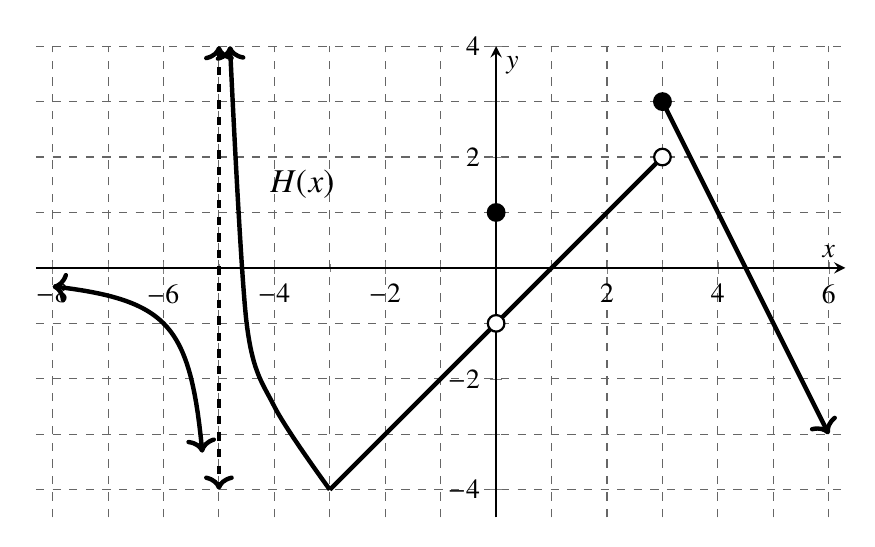
\begin{tikzpicture}
\begin{axis}[scale=1.5, thick, my style, xtick={-8,-6,-4,-2,...,6}, ytick={-6, -4,-2,0,2,4},
xmin=-8.3, xmax=6.3, ymin=-4.5, ymax=4, minor y tick num=1,
        minor x tick num=1, mark size=3.0pt, grid=both, grid style={ thin, black!60, dashed}, axis equal image]
% %%asymptote
\addplot[dashed,<->, ultra thick] coordinates {(-5,4) (-5,-4)};       
%%%points solid
\addplot[mark=*,only marks] coordinates {(0,1) (3,3)};
%%%points open
\addplot[mark=*,fill=white,only marks] coordinates {(0,-1)(3,2)};
%%%Curves
%%\addplot[ultra thick, smooth, ->] coordinates {(-5,2)(-4,1)(-3,1.1)(-2.3,3)(-2.1,6.2)};
\addplot[ultra thick, smooth] coordinates {(-3,-4) (3,2)};
\addplot[ultra thick, smooth, ->] coordinates {(3,3) (6,-3)};
% \addplot[->,ultra thick, smooth, variable=\x, samples=100, domain=1:6] plot(\x,{(-0.15)*(\x -1)*(\x -1)+5});  
\addplot[ultra thick, <->,domain=-8:-5.3, samples=100]{1/(x+5)}; 
\addplot[ultra thick, smooth, ->] coordinates {(-3,-4)(-4, -2.5)(-4.5,-1)(-4.8, 4)}; 
%\addplot[ultra thick, smooth, ] coordinates {(1,1)(3,1)}; 
%\addplot[ultra thick, smooth, -] (-2,2) parabola  (1,-1);
\node at (-3.5,1.5){\large{$H(x)$}};
\end{axis}

\end{tikzpicture}
\end{center}

\newcommand{\ans}{\blank{1cm}}

\begin{subproblems}
{\setstretch{2}
\item What is the \emph{domain} of $H(x)$? Write your answer in \emph{interval notation}.

domain = \blank{3in}

\begin{multicols}{3}
%\begin{tabular}{c c c}
\item $\ds{\lim_{x \to -5^{-}} H(x)} = $ \ans 
\item $\ds{\lim_{x \to -5^{+}} H(x)} = $ \ans 
\item $\ds{\lim_{x \to -5} H(x)} = $ \ans 
%
%\columnbreak
\item $\ds{\lim_{x \to 3^{-}} H(x)} = $ \ans
%
\item $\ds{\lim_{x \to 3^{+}} H(x)} = $ \ans
\item $H(3)=$ \ans
\item $H'(4) = $ \ans
\item $H(0)= $ \ans
%\columnbreak
\item $\ds{\lim_{x \to 0} H(x)} = $ \ans
\item $\ds{\lim_{x \to -3} H(x)} = $ \ans
\item $H(-3) = $\ans

\end{multicols}
%\end{tabular}

%\bigskip



\item Is $H'(-3)$ defined? Why or why not? Explain your answer in a few words.

\vspace{2cm}
}
\item List the values of $x$ in the interval $(-\infty, \infty)$ where $H(x)$ is NOT continuous. If $H(x)$ is continuous everywhere, write ``none''.

\bigskip

$x = \blank{3in}$



\end{subproblems}


\newpage


%%%%%% Compute the limits

\problem{12 points} Compute the following limits. Show your work. Use limit notation where necessary; you will be graded both on your computation and on your correct use of notation.

If the limit does not exist, write {\bf DNE} and a few words about why it does not exist. If the limit increases without bound, write $\infty$ or $-\infty$.
%
\begin{subproblems}
\item \ 
$\ds{\lim_{x\to 3} \frac{e^{x} + 4}{x-8} } = $
%
\vfill
%
\item $\ds{\lim_{t \to 2^{-}} \frac{(t+2)(t+3)}{t(t-2)}} = $
%
\vfill
%
\item $\ds{\lim_{h \to 0} \frac{\sqrt{x+h} - \sqrt{x}}{h}  }= $
%
\vfill
%
\item A function $\ds f(x)$ has been numerically evaluated as follows:

\begin{tabular}{|c|| c| c |c || c | c | c|}
\hline
$x$&1.001 & 1.0001 & 1.00001 & 0.99999& 0.9999 & 0.999\\ \hline
$f(x)$ & 1.50150 & 1.50015 & 1.50002 & 1.49999 &  1.49985 & 1.49850 \\ \hline
\end{tabular}

\bigskip

Estimate $\ds{\lim_{x\to 1} f(x)  = }$ \ans\ans\ans

%$\ds{\lim_{x\to 2^{-}} \frac{2x^{2}-x-3}{4x-8}}$
%
%\vfill

\end{subproblems}

\newpage

%%% Definition of the derivative
\problem{10 points}
%\begin{subproblems}
%\item Suppose $f(x)$ is a function. State the limit definition of the derivative $f'(x)$.
%\vspace{1in}


 Consider the function
 \[\displaystyle f(x)=\frac{3}{x^2}+7.\] %\[\displaystyle f(x)=\frac{1}{6-x}.\] 

Find $f'(2)$ %$f'(5)$
 using the \emph{limit definition of the derivative} and show your work using all appropriate notation. 

No credit will be awarded for using other methods. Begin by writing down the limit definition of the derivative. You must write limits where necessary to receive full credit. 
%\ee
\vfill

%\end{subproblems}
\newpage

%%% Function and derivative interpretation

\problem{12 points} 
 A certain population of rabbits can be modeled by a function $P(t)$, where $t$ measures time, in years, since 2018.

\begin{subproblems}
\item Suppose you are told that $P(5) = 285$. Write a sentence explaining what this means in the context of the problem, and use units in your answer.

\vfill

\item Suppose, in addition, you are told that $P(0) = 20$. What is the average rate of population change between 2018 and 2023? Do a computation to determine this quantity, and write your answer in a sentence, including units.

\vfill

\item The quantity $P'(5) = 85$. Write a sentence explaining what this means in the context of the problem, and include units in your answer.

\vfill

\item Suppose that $P'(t) < 0$ for $t \geq 8$. Write a sentence explaining what this means in the context of the problem.

\vfill

\end{subproblems}



\newpage



%%%%% Derivatives and tangent lines
\problem{12 points} Consider the function 
%$\displaystyle{f(x) = \frac{3x^2}{x^2 +2}}$ 
$\ds g(x) = %(x+1)^{2}(x+4) + 6$
x^3+6 x^2+9 x+10$
whose graph is shown below.


\begin{center} 

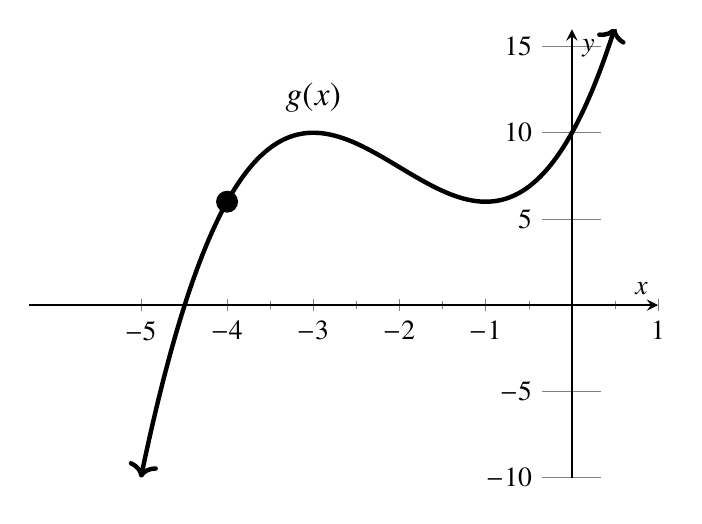
\begin{tikzpicture}
\begin{axis}[xscale=5, yscale = 1, thick, my style, xtick={-5, -4,-3, -2,...,1}, ytick={-10,-5,...,15},
xmin=-6.3, xmax=1, ymin=-10, ymax=16, minor y tick num=0,
        minor x tick num=1, mark size=3.0pt, grid=none, grid style={ thin, black!60}, axis equal image]
% %%asymptote
%\addplot[dashed,<->, ultra thick] coordinates {(5,-4) (5,4)};       
%%%points solid
%\addplot[mark=*,only marks] coordinates {(-4,6)};
%%%points open
%\addplot[mark=*,fill=white,only marks] coordinates {(-2,2)(1,1)(1,-1)(3,-3)};
%%%Curves
%%\addplot[ultra thick, smooth, ->] coordinates {(-5,2)(-4,1)(-3,1.1)(-2.3,3)(-2.1,6.2)};
%\addplot[ultra thick, smooth] coordinates {(-5,-2) (-2,2)};
\addplot[<->,ultra thick, smooth, variable=\x, samples=100, domain=-5:.5] plot(\x,{(\x+1)*(\x+1)*(\x+4)+6)});   
%\addplot[ultra thick, smooth, ->] coordinates {(3,-3)(4, -2.5)(4.5,-1)(4.8, 4)}; 
%\addplot[ultra thick, smooth, ] coordinates {(1,1)(3,1)}; 
%\addplot[ultra thick, smooth, -] (-2,2) parabola  (1,-1);
\node at (-3,12){\large{$g(x)$}};
\draw[fill= black] (-4,6) circle (.25mm and 1.25mm);
\end{axis}

\end{tikzpicture}
\end{center}
%\begin{tikzpicture}[scale = .8]%[background color=orange!10,use background]
%Grid 
%\draw[step = 1 cm, gray, very thin] (-7, -2) grid (8,4); % Another way to make grids
%
%%x-axis
%\draw[very thick, ->] (-7,0) -- (8,0) node[anchor = north west] {$x$};
%
%%y-axis
%\draw[very thick, ->] (0,-4) -- (0,4) node[anchor = south east] {$y$};
%
%%labels on x-axis
%\foreach \x in {-4,...,7}
%  \draw (\x cm, 1pt) -- (\x cm, -1pt) node[anchor = north] {$\x$};
%
%%labels on y-axis
%\foreach \y in {-2,..., 4}
%\draw (1pt, \y cm) -- (-1pt, \y cm) node[anchor = east] {$\y$};
%
%%function graph  \x for x  on [-7,6] 
%\draw[black, line width=.75mm, samples=40, <->] 
%      plot[domain=-7:6] 
%      (\x,{(\x+1)*(\x+1)*(\x+4)+6)});

%function graph  \x for x  on [2,8] 
%\draw[black, line width=.75mm, samples=100, <->] 
 %    plot[domain=2.13:8] 
  %  (\x,{(0.1*\x*\x)/(\x -2)});

%Vertical dashed colored line
%\draw [dashed, very thick] (-7,3) -- (7,3);

% Draw (2,2) with dot
%\fill (2,2) circle[radius=4pt];

%\end{tikzpicture}
%\end{center}

\begin{subproblems}
%\be
\item Draw and \emph{label} (with the word ``tangent'') the tangent line to the graph at the point $(-4, g(-4)) = (-4,6)$ shown on the graph.
  \item Find $g'(x)$. %Use whatever method you like. Show your work. 
  (You do not need to use the limit definition of the derivative to answer this problem.)
  
  \vfill %
%  \vspace{3cm}
%  \item Use your answer from part (a) to determine the slope of the line tangent to $f(x)$ at the point $P(2,2)$.
%  \vspace{2cm}
  \item Write down an equation for the tangent line at the point $(-4,6)$. Your equation should use point-slope form: that is, it should be of the form $y = m(x-x_{1})+y_{1}$.
  
  
    \vfill
    
  equation of tangent line: \hrulefill
  
  \item Do a computation to determine (exactly) the $x$-coordinates of all points on the graph where there is a horizontal tangent line. Show your work.
  
  \vfill
  
  \vfill
  
  \vfill




\end{subproblems}
%\ee

\newpage

\problem{8 points} Match the graph of each function (a) -- (d) with the graph of its derivative, chosen from the list of graphs I -- IX. Write your answer in the blanks below.

\hrulefill

\emph{Your answers:}
 
 \emph{i.} The derivative of graph (a) is \ans. \hfill  \emph{ii.} The derivative of graph (b) is \ans.
 
  \emph{iii.} The derivative of graph (c) is \ans. \hfill  \emph{iv.} The derivative of graph (d) is \ans.
 
 \hrulefill
 
 \emph{The graphs:}
 
 \def\rr{.25}

{\centering
\begin{tabular}{c c}
(a) \resizebox{\rr\linewidth}{!}{
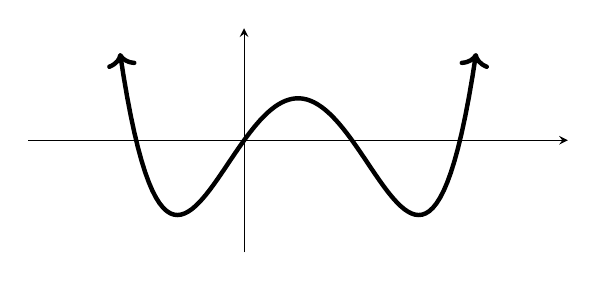
\begin{tikzpicture}
\begin{axis}[%x=1cm,y=1cm,scale=0.5,xscale=1.5, thick, 
my style, 
yscale = .5,
xlabel={\empty},ylabel={\empty},
xtick={\empty}, ytick={\empty},
xticklabel = {\empty}, yticklabel={\empty},
xmin=-2, xmax=3, ymin=-.5, ymax=.5, 
%mark size=3.0pt, grid = major
]
\addplot[ultra thick, <->,domain=-1.15:2.15, samples=100]{(x - 1)*(x + 1)*x*(x - 2)/3};
\end{axis}
\end{tikzpicture}
}
%%%%
&
(b)  \resizebox{\rr\linewidth}{!}{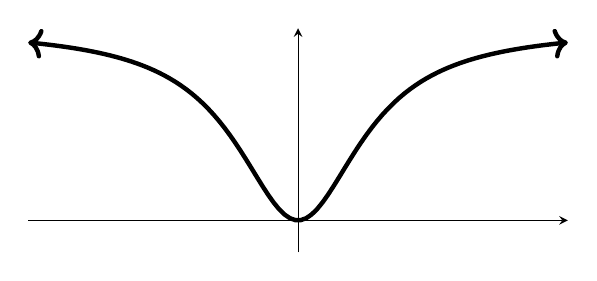
\begin{tikzpicture}
\begin{axis}[%x=1cm,y=1cm,
yscale=0.5,
xscale=1, %thick, 
my style, 
xlabel={\empty},ylabel={\empty},
xtick={\empty}, ytick={\empty},
xticklabel = {\empty}, yticklabel={\empty},
xmin=-5, xmax=5, ymin=-.5, ymax=3, 
%mark size=3.0pt, grid = major
]
\addplot[ultra thick, <->,domain=-5:5, samples=100]{3*x*x/(x*x+2)};
\end{axis}
\end{tikzpicture}
}
\\
%%

(c)  \resizebox{\rr\linewidth}{!}{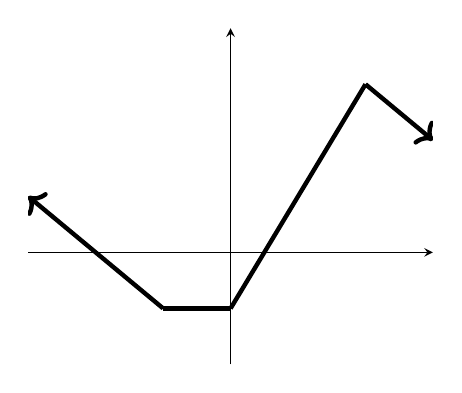
\begin{tikzpicture}
\begin{axis}[%x=1cm,y=1cm,
yscale=.75,
xscale=.75, %thick, 
my style, 
xlabel={\empty},ylabel={\empty},
xtick={\empty}, ytick={\empty},
xticklabel = {\empty}, yticklabel={\empty},
xmin=-3, xmax=3, ymin=-2, ymax=4, 
%mark size=3.0pt, grid = major
]
\addplot[ultra thick, <-,domain=-3:-1, samples=100]{-2-x};
\addplot[ultra thick, -,domain=-1:0, samples=100]{-1};
\addplot[ultra thick, -,domain=0:2, samples=100]{2*x-1};
\addplot[ultra thick, ->,domain=2:3, samples=100]{5-x};

\end{axis}
\end{tikzpicture}
}
%%%%%%%%%
&
%%%%%%%%
(d)  \resizebox{\rr\linewidth}{!}{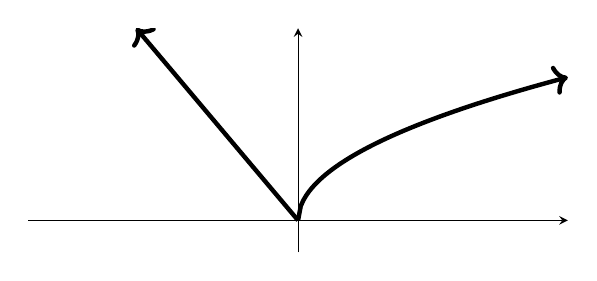
\begin{tikzpicture}
\begin{axis}[%x=1cm,y=1cm,
yscale=0.5,
xscale=1, %thick, 
my style, 
xlabel={\empty},ylabel={\empty},
xtick={\empty}, ytick={\empty},
xticklabel = {\empty}, yticklabel={\empty},
xmin=-5, xmax=5, ymin=-.5, ymax=3, 
%mark size=3.0pt, grid = major
]
\addplot[ultra thick, ->,domain=0:5, samples=100]{sqrt(x)};
\addplot[ultra thick, <-,domain=-3:0, samples=100]{-x};

\end{axis}
\end{tikzpicture}
}
%%%%%%%%%%%


\end{tabular}

}

\hrulefill

\emph{Possible derivatives:}

\def\r{.22}

%\begin{tabular}{c c c}
I. 
\resizebox{\r\linewidth}{!}{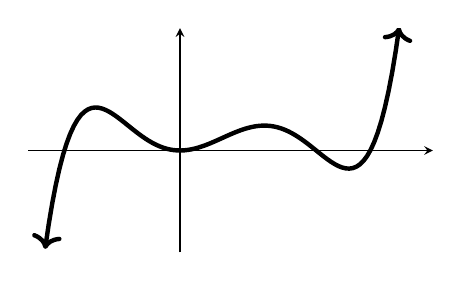
\begin{tikzpicture}
\begin{axis}[%x=1cm,y=1cm,scale=0.5,xscale=1.5, thick, 
my style, 
yscale = .5,
xscale = .75,
xlabel={\empty},ylabel={\empty},
xtick={\empty}, ytick={\empty},
xticklabel = {\empty}, yticklabel={\empty},
xmin=-1.8, xmax=3, ymin=-.5, ymax=.6, 
%mark size=3.0pt, grid = major
]
\addplot[ultra thick, <->,domain=-1.6:2.6, samples=100]{1/90*x^2*(30-10*x-15*x^2+6*x^3)};
\end{axis}
\end{tikzpicture}
}
%
\hfill
II. 
 \resizebox{\r\linewidth}{!}{\begin{tikzpicture}
\begin{axis}[%x=1cm,y=1cm,
yscale=.75,
xscale=.75, %thick, 
my style, 
xlabel={\empty},ylabel={\empty},
xtick={\empty}, ytick={\empty},
xticklabel = {\empty}, yticklabel={\empty},
xmin=-3, xmax=3, ymin=-2, ymax=4, 
%mark size=3.0pt, grid = major
]
\addplot[ultra thick, <-,domain=-3:-1, samples=100]{-1};
\addplot[ultra thick, -,domain=-1:0, samples=100]{0};
\addplot[ultra thick, -,domain=0:2, samples=100]{2};
\addplot[ultra thick, ->,domain=2:3, samples=100]{-1};
\draw[black, fill = white] (-1,-1) circle (1mm);
\draw[black, fill = white] (-1,0) circle (1mm);
\draw[black, fill = white] (0,0) circle (1mm );
\draw[black, fill = white] (0,2) circle (1mm);
\draw[black, fill = white] (2,2) circle (1mm );
\draw[black, fill = white] (2,-1) circle (1mm );

\end{axis}
\end{tikzpicture} 
}
%
\hfill
%%%%%%%%%
%
III.
\resizebox{\r\linewidth}{!}{
\begin{tikzpicture}
\begin{axis}[%x=1cm,y=1cm,
yscale=.75,
xscale=.75, %thick, 
my style, 
xlabel={\empty},ylabel={\empty},
xtick={\empty}, ytick={\empty},
xticklabel = {\empty}, yticklabel={\empty},
xmin=-3, xmax=3, ymin=-2, ymax=4, 
%mark size=3.0pt, grid = major
]
\addplot[ultra thick, <-,domain=-3:-1, samples=100]{1};
\addplot[ultra thick, -,domain=-1:0, samples=100]{-1};
\addplot[ultra thick, -,domain=0:2, samples=100]{2};
\addplot[ultra thick, ->,domain=2:3, samples=100]{1};
\draw[black, fill = white] (-1,1) circle (1mm);
\draw[black, fill = white] (-1,-1) circle (1mm);
\draw[black, fill = white] (0,-1) circle (1mm );
\draw[black, fill = white] (0,2) circle (1mm);
\draw[black, fill = white] (2,2) circle (1mm );
\draw[black, fill = white] (2,1) circle (1mm );
\end{axis}
\end{tikzpicture} 
}


%%%%%%%%%%%%%%%
IV. \resizebox{\r\linewidth}{!}{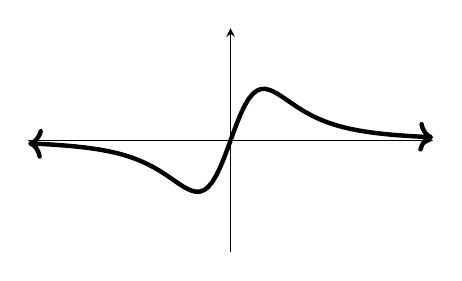
\begin{tikzpicture}
\begin{axis}[%x=1cm,y=1cm,
yscale=0.5,
xscale=.75, %thick, 
my style, 
xlabel={\empty},ylabel={\empty},
xtick={\empty}, ytick={\empty},
xticklabel = {\empty}, yticklabel={\empty},
xmin=-5, xmax=5, ymin=-3, ymax=3, 
%mark size=3.0pt, grid = major
]
\addplot[ultra thick, <->,domain=-5:5, samples=100]{12*x/((x^2+2)*(x^2+2))};
\end{axis}
\end{tikzpicture}
}
%%%
\hfill
V. 
 \resizebox{\r\linewidth}{!}{
 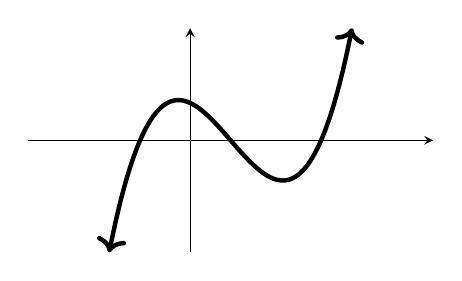
\begin{tikzpicture}
\begin{axis}[%x=1cm,y=1cm,scale=0.5,xscale=1.5, thick, 
my style, 
yscale = .5,
xscale = .75,
xlabel={\empty},ylabel={\empty},
xtick={\empty}, ytick={\empty},
xticklabel = {\empty}, yticklabel={\empty},
xmin=-2, xmax=3, ymin=-3, ymax=3, 
%mark size=3.0pt, grid = major
]
\addplot[ultra thick, <->,domain=-1:2, samples=100]{2/3 (1 - x - 3*x^2 + 2*x^3)};
\end{axis}
\end{tikzpicture}
}
%%%%%%%
\hfill
VI. 
\resizebox{\r\linewidth}{!}{
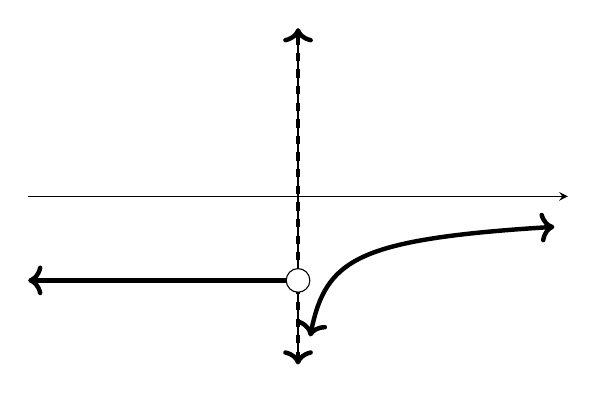
\begin{tikzpicture}
\begin{axis}[%x=1cm,y=1cm,
yscale=.75,
xscale=1, %thick, 
my style, 
xlabel={\empty},ylabel={\empty},
xtick={\empty}, ytick={\empty},
xticklabel = {\empty}, yticklabel={\empty},
xmin=-2, xmax=2, ymin=-2, ymax=2, 
%mark size=3.0pt, grid = major
]
\addplot[ultra thick, <->,domain=.09:1.9, samples=100]{-1/(2*sqrt(x))};
\addplot[ultra thick, <-,domain=-2:0, samples=100]{-1};
%\addplot[mark=*,fill=white,only marks] coordinates {(0,-1)};
\draw[ultra thick, dashed, <->] (0,-2) -- (0,2);
\draw[black, fill = white] (0,-1) circle (1.5mm and 2 mm);

\end{axis}
\end{tikzpicture}
}
%

VII. 
\resizebox{\r\linewidth}{!}{
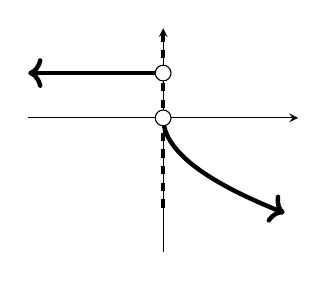
\begin{tikzpicture}
\begin{axis}[%x=1cm,y=1cm,
yscale=.5,
xscale=.5, %thick, 
my style, 
xlabel={\empty},ylabel={\empty},
xtick={\empty}, ytick={\empty},
xticklabel = {\empty}, yticklabel={\empty},
xmin=-5, xmax=5, ymin=-3, ymax=2, 
%mark size=3.0pt, grid = major
]
\addplot[ultra thick, ->,domain=0:4.5, samples=100]{-sqrt(x))};
\addplot[ultra thick, <-,domain=-5:0, samples=100]{1};
%\addplot[mark=*,fill=white,only marks] coordinates {(0,-1)};
\draw[ultra thick, dashed] (0,-2) -- (0,3);
\draw[black, fill = white] (0,1) circle (2mm and 2mm);
\draw[black, fill = white] (0,0) circle (2mm and 2mm);
\end{axis}
\end{tikzpicture}
}
%%%%%
\hfill
VIII. 
\resizebox{\r\linewidth}{!}{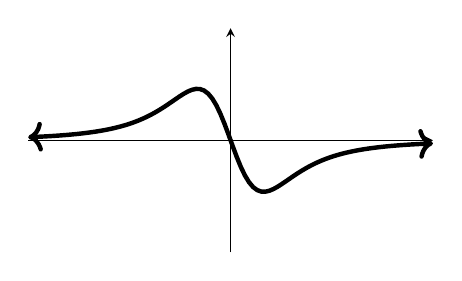
\begin{tikzpicture}
\begin{axis}[%x=1cm,y=1cm,
yscale=0.5,
xscale=.75, %thick, 
my style, 
xlabel={\empty},ylabel={\empty},
xtick={\empty}, ytick={\empty},
xticklabel = {\empty}, yticklabel={\empty},
xmin=-5, xmax=5, ymin=-3, ymax=3, 
%mark size=3.0pt, grid = major
]
\addplot[ultra thick, <->,domain=-5:5, samples=100]{-12*x/((x^2+2)*(x^2+2))};
\end{axis}
\end{tikzpicture}
}
%%%%%%%%%%%
\hfill
IX.
 \resizebox{\r\linewidth}{!}{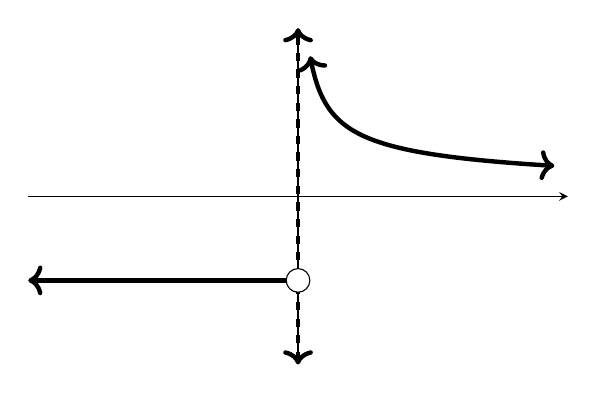
\begin{tikzpicture}
\begin{axis}[%x=1cm,y=1cm,
yscale=.75,
xscale=1, %thick, 
my style, 
xlabel={\empty},ylabel={\empty},
xtick={\empty}, ytick={\empty},
xticklabel = {\empty}, yticklabel={\empty},
xmin=-2, xmax=2, ymin=-2, ymax=2, 
%mark size=3.0pt, grid = major
]
\addplot[ultra thick, <->,domain=.09:1.9, samples=100]{1/(2*sqrt(x))};
\addplot[ultra thick, <-,domain=-2:0, samples=100]{-1};
%\addplot[mark=*,fill=white,only marks] coordinates {(0,-1)};
\draw[ultra thick, dashed, <->] (0,-2) -- (0,2);
\draw[black, fill = white] (0,-1) circle (1.5mm and 2 mm);

\end{axis}
\end{tikzpicture}
}


%\end{tabular}

%A function $g(x)$ is shown. Sketch the derivative $g'(x)$ on the second set of axes. Indicate any asymptotes the derivative might have using dashed lines, and indicate any points where the derivative is undefined using open circles.

%%%%SKETCH DERIVATIVE FROM GRAPH OF FUNCTION
%\item (16 points) Use the graph of $g(x)$, in the figure below, to answer the questions (a)-(g). The dashed lines in the figure represent asymptotes of the graph of $g(x).$ 
%\begin{multicols}{3}
%%%%Begin FIGURE
%\begin{center}
%%%G
%\begin{tikzpicture}
%\begin{axis}[x=1cm,y=1cm,scale=0.5,xscale=1.5, thick, my style, xtick={-7,-6,...,8,9}, ytick={1,...,6,7,8},xmin=-7.9, xmax=10, ymin=-1.5, ymax=8, mark size=3.0pt, grid = major]
%\addplot[ultra thick, ,] coordinates {(-6,5) (-2,5)};
%\addplot[ultra thick, ,] coordinates {(-2,5) (2, 3)};
%\addplot[ultra thick, ,]  (2,3) parabola bend (5,6) (9,1);
%%\addplot[dashed, thick,<->] coordinates {(-7.5,6) (10,6)};
%%\addplot[ultra thick, ->,domain=2:10, samples=100]{6-4/(x-1)};
%%\addplot[ultra thick, domain=-4:2, samples=100]{3-0.5*(x)};
%%\addplot[ultra thick, domain=-7.8:-4.17, samples=100,<->]{6+0.5/(x+4.1)};
%\node at (-4,6){\large{$g(x)$}};
%%\draw[fill=black, thick] (-4,5) circle  (1.2 mm);
%\end{axis}
%\end{tikzpicture}
%
%\bigskip
%
%%%G' location
%\begin{tikzpicture}
%\begin{axis}[x=1cm,y=1cm,scale=0.5,xscale=1.5, thick, my style, xtick={-7,-6,...,8,9}, ytick={0},%{1,...,6,7,8},
%xmin=-7.9, xmax=10, ymin=-5, ymax=5, mark size=3.0pt, grid = none, x tick style = {black, thick}]
%%\addplot[ultra thick, ,] coordinates {(-6,5) (-2,5)};
%%\addplot[ultra thick, ,] coordinates {(-2,5) (2, 3)};
%%\addplot[ultra thick, ,]  (2,3) parabola bend (5,6) (9,1);
%%\addplot[dashed, thick,<->] coordinates {(-7.5,6) (10,6)};
%%\addplot[ultra thick, ->,domain=2:10, samples=100]{6-4/(x-1)};
%%\addplot[ultra thick, domain=-4:2, samples=100]{3-0.5*(x)};
%%\addplot[ultra thick, domain=-7.8:-4.17, samples=100,<->]{6+0.5/(x+4.1)};
%%\node at (-4,6){\large{$g(x)$}};
%%\draw[fill=black, thick] (-4,5) circle  (1.2 mm);
%\end{axis}
%\end{tikzpicture}
%\end{center}

%%%% End FIGURE


%%%%% Another derivatives and tangent lines problem, this time with algebra.
%\problem{10} 
%\problem{8 points} Consider the function $\displaystyle{f(x) = 2\sin x -x}$. Determine all $x$-values on the interval $[0,2\pi]$ for which $f(x)$ has a {\bf horizontal tangent line}.


%\begin{center}
%\begin{tikzpicture}%[background color=orange!10,use background]
%  \begin{axis}%
%    [grid=both,
%     minor tick num=4,
%     grid style={line width=.1pt, draw=gray!4},
%     major grid style={line width=.2pt,draw=gray!50},
%     axis lines=middle,
%     enlargelimits={abs=0.2}
%    ]
%    \addplot[domain=-10:10,samples=50,smooth,blue, line width=2pt] {2*sin(deg(x)) -x};
%  \end{axis}
%\end{tikzpicture}
%\end{center}

\vspace{2in}

\newpage



%%%%%% Continuity and piecewise functions

%\problem{10} %%%% UPDATED 2024
\problem{10 points} Let 
{\setstretch{2}
\[f(x)=\begin{cases} \ds{\frac{4^x}{x+x^2}} & x < 1\\1 & x=1 \\ \ds{\frac{2-2x}{x-x^2}} & x > 1 \end{cases}\]
}

\begin{subproblems}
	\item Evaluate $\ds{ \lim_{x \to 1^-} f(x)}$. Show supporting work, including correct use of limit notation.
	%\vspace{.7in}
	\vfill
	\item Evaluate $\ds{ \lim_{x \to 1^+} f(x)}$. Show supporting work, including correct use of limit notation.
	%\vspace{.7in} 
	\vfill
	\item Evaluate $f(1)$. 
	\vspace{.5in}
	\item Based on your answers to parts (a), (b) and (c), \emph{check the true statement(s) below}:
	\begin{enumerate}[$\Box$]
		\item $f$ is continuous at $x=0$.
		\item $f$ has a removable discontinuity at $x=0$.
		\item $f$ has a jump discontinuity at $x=0$.
		\item $f$ has an infinite discontinuity at $x=0$.
		\item None of the above.
	\end{enumerate}
	\vspace{.2in}
\end{subproblems}


\newpage


%%%%% Compute the derivative

%\problem{18} %%%%%%UPDATED FOR 2024

\problem{12 points} For each of the following functions, compute the derivative. 
\emph{You do not need to simplify your answers.} Your answer must begin with $f'(x), \frac{df}{dx}, \frac{dy}{dx}, y'$, or similar notation, as appropriate to the problem.
 
\begin{subproblems}

\item $\displaystyle{f(x) = x^6 - 7x^4 + \frac{1}{x^2} + \cos(2)}$
\vfill
 
\item $\displaystyle{g(\theta) = (2\theta+\pi)\sin(\theta)}$ %% product rule
  
\vfill
  
\item $\displaystyle{h(t) = \frac{t^\frac{5}{2}+t-4}{\sqrt{t}}}$ %% quotient rule or cleverness
  
\vfill  

\item $\ds k(x) = \frac{3x^{2}}{x^{2}+2}$

\vfill



\end{subproblems}


\newpage



%%%%%%%%%% velocity and stuff


\problem{8 points} A particle moves back and forth along a coordinate axis in such a way that its \emph{position} at time $t$ is given by the function 
\[ s(t) = t - \cos(t).\]
The position of the particle is measured in millimeters, and time is measured in seconds.
\begin{subproblems}

\item Determine the velocity function $v(t)$ and the acceleration function $a(t)$ of the particle.

\vfill

\item What is the initial velocity of the particle? Give units in your answer.

\vfill

\item At time $t = \frac{\pi}{6}$ is the particle speeding up or slowing down? Explain how you know with a computation and some words.

\vfill

\item On the time interval $[0, \pi]$,  does the particle ever stop? Explain your answer with a computation and some words.

\vfill

\end{subproblems}

\newpage

%\end{enumerate}
%%%%%%%%%%%%%%%%%%%%%%%%%%%

%\fbox{Extra Credit} 
\emph{Extra Credit: }(5 points) Consider the function $\displaystyle f(x)=\frac{2^x}{1-x}$.\\
\begin{enumerate}[i.]
\item What is $f(0)$?
\vspace{1in}
\item What is $f(3)$?
\vspace{1in}
\item Can we use the Intermediate Value Theorem to conclude that $f(x) = 0$ for some $x$ in the interval $[0,3]$? If so, write an explanation for how the Intermediate Value Theorem lets us conclude this. If not, explain why not.
\vfill
\end{enumerate}

\vfill



\vfill

\end{document}

%%%%ENDDOCUMENT


